\documentclass[12pt,a4paper,openany]{book}

\usepackage{lmodern}
\usepackage{xcolor}
\usepackage{xcolor}
\definecolor{vert1}{rgb}{0.0,0.3.9,0.0}
\definecolor{bleu}{rgb}{0,0,0.5}
\definecolor{bleu3}{rgb}{1,0.2,0.2}
\definecolor{grisgris}{gray}{0.4}
\definecolor{grisclair}{HTML}{E7E7E7}
\definecolor{grisfonce}{HTML}{A5A5A5}
\definecolor{rougeUPS}{rgb}{0.6, 0.3, 0.3}

\fboxsep =0pt \parindent =0pt\parskip =12pt



\usepackage[utf8]{inputenc}
\usepackage[T1]{fontenc}
\usepackage[francais]{babel}
\usepackage[top=1.7cm, bottom=1.7cm, left=1.7cm, right=1.7cm]{geometry}
\usepackage{verbatim}
\usepackage[urlbordercolor={1 1 1}, linkbordercolor={1 1 1}, linkcolor=vert1, urlcolor=bleu, colorlinks=true]{hyperref}
\usepackage{tikz} %Vectoriel
\usepackage{listings}
\usepackage{fancyhdr}
\usepackage{multido}
\usepackage{amssymb}
\usepackage{float}

\newcommand{\titre}{Algorithmie en langage C}

\newcommand{\pole}{}
\newcommand{\sigle}{algo}

\newcommand{\semestre}{3}

\definecolor{gris1}{gray}{0.40}
\definecolor{gris2}{gray}{0.55}
\definecolor{gris3}{gray}{0.65}
\definecolor{gris4}{gray}{0.50}
\definecolor{vert}{rgb}{0,0.4,0}
\definecolor{violet}{rgb}{0.65, 0.2, 0.65}
\definecolor{bleu1}{rgb}{0,0,0.8}
\definecolor{bleu2}{rgb}{0,0.2,0.6}
\definecolor{bleu3}{rgb}{0,0.2,0.2}
\definecolor{rouge}{HTML}{F93928}


\lstdefinelanguage{algo}{%
   morekeywords={%
    %%% couleur 1
		importer, programme, glossaire, fonction, procedure, constante, type, 
	%%% IMPORT & Co.
		si, sinon, alors, fin, tantque, debut, faire, lorsque, fin lorsque, 
		declenche, declencher, enregistrement, tableau, retourne, retourner, =, pour, a,
		/=, <, >, traite,exception, 
	%%% types 
		Entier, Reel, Booleen, Caractere, Réél, Booléen, Caractère,
	%%% types 
		entree, maj, sortie,entrée,
	%%% types 
		et, ou, non,
	},
  sensitive=true,
  morecomment=[l]{--},
  morestring=[b]',
}

\lstset{language=algo,
    %%% BOUCLE, TEST & Co.
      emph={importer, programme, glossaire, fonction, procedure, constante, type},
      emphstyle=\color{bleu2},
    %%% IMPORT & Co.  
	emph={[2]
		si, sinon, alors, fin , tantque, debut, faire, lorsque, fin lorsque, 
		declencher, retourner, et, ou, non,enregistrement, retourner, retourne, 
		tableau, /=, <, =, >, traite,exception, pour, a
	},
      emphstyle=[2]\color{bleu1},
    %%% FONCTIONS NUMERIQUES
      emph={[3]Entier, Reel, Booleen, Caractere, Booléen, Réél, Caractère},
      emphstyle=[3]\color{gris1},
    %%% FONCTIONS NUMERIQUES
      emph={[4]entree, maj, sortie, entrée},	
      emphstyle=[4]\color{gris1},
}
\lstdefinelanguage{wl}{%
   morekeywords={%
    %%% couleur 1
		importer, programme, glossaire, fonction, procedure, constante, type, 
	%%% IMPORT & Co.
		si, sinon, alors, fin, TANTQUE, tantque, FIN, PROCEDURE, debut, faire, lorsque, 
		fin lorsque, declenche, declencher, enregistrement, tableau, retourne, retourner, =, 
		/=, <, >, traite,exception, 
	%%% types 
		Entier, Reel, Booleen, Caractere, Réél, Booléen, Caractère,
	%%% types 
		entree, maj, sortie,entrée,
	%%% types 
		et, ou, non,
	},
  sensitive=true,
  morecomment=[l]{//},
  morestring=[b]',
}

\lstset{language=wl,
    %%% BOUCLE, TEST & Co.
      emph={importer, programme, glossaire, fonction, procedure, constante, type},
      emphstyle=\color{bleu2},
    %%% IMPORT & Co.  
	emph={[2]
		si, sinon, alors, fin , tantque, debut, faire, lorsque, fin lorsque, 
		declencher, retourner, et, ou, non,enregistrement, retourner, retourne, 
		tableau, /=, <, =, >, traite,exception
	},
      emphstyle=[2]\color{bleu1},
    %%% FONCTIONS NUMERIQUES
      emph={[3]Entier, Reel, Booleen, Caractere, Booléen, Réél, Caractère},
      emphstyle=[3]\color{gris1},
    %%% FONCTIONS NUMERIQUES
      emph={[4]entree, maj, sortie, entrée},	
      emphstyle=[4]\color{gris1},
}
\lstdefinelanguage{css}{%
   morekeywords={%
    %%% couleur 1
		background, image, repeat, position, index, color, border, font, 
		size, url, family, style, variant, weight, letter, spacing, line, 
		height, text, decoration, align, indent, transform, shadow, 
		background, image, repeat, position, index, color, border, font, 
		size, url, family, style, variant, weight, letter, spacing, line, 
		height, text, decoration, align, indent, transform, shadow, 
		vertical, align, white, space, word, spacing,attachment, width, 
		max, min, margin, padding, clip, direction, display, overflow,
		visibility, clear, float, top, right, bottom, left, list, type, 
		collapse, side, empty, cells, table, layout, cursor, marks, page, break,
		before, after, inside, orphans, windows, azimuth, after, before, cue, 
		elevation, pause, play, during, pitch, range, richness, spek, header, 
		numeral, punctuation, rate, stress, voice, volume,
	%%% types 
		left, right, bottom, top, none, center, solid, black, blue, red, green,
	},
  sensitive=true,
  sensitive=true,
  morecomment=[s]{/*}{*/},
  morestring=[b]',
}
\lstset{language=css,
    %%% BOUCLE, TEST & Co.
      emph={
		background, image, repeat, position, index, color, border, font, 
		size, url, family, style, variant, weight, letter, spacing, line, 
		height, text, decoration, align, indent, transform, shadow, 
		background, image, repeat, position, index, color, border, font, 
		size, url, family, style, variant, weight, letter, spacing, line, 
		height, text, decoration, align, indent, transform, shadow, 
		vertical, align, white, space, word, spacing,attachment, width, 
		max, min, margin, padding, clip, direction, display, overflow,
		visibility, clear, float, top, right, bottom, left, list, type, 
		collapse, side, empty, cells, table, layout, cursor, marks, page, break,
		before, after, inside, orphans, windows, azimuth, after, before, cue, 
		elevation, pause, play, during, pitch, range, richness, spek, header, 
		numeral, punctuation, rate, stress, voice, volume,
	  },
      emphstyle=\color{bleu2},
    %%% FONCTIONS NUMERIQUES
      emph={[3]
		left, right, bottom, top,none, solid, black, blue, green,
		  },
      emphstyle=[3]\color{bleu3},
    %%% FONCTIONS NUMERIQUES
}

\lstset{language=SQL,
    %%% BOUCLE, TEST & Co.
      emph={INSERT, UPDATE, DELETE, WHERE, SET, GROUP, BY, ORDER, REFERENCES},
      emphstyle=\color{bleu2},
    %%% IMPORT & Co.  
	emph={[2]
		if, end, begin, then, for, each, else, after, of, on, to
	},
      emphstyle=[2]\color{bleu1},
    %%% FONCTIONS NUMERIQUES
      emph={[3]Entier, Reel, Booleen, Caractere, Booléen, Réél, Caractère},
      emphstyle=[3]\color{gris1},
    %%% FONCTIONS NUMERIQUES
      emph={[4]entree, maj, sortie, entrée},	
      emphstyle=[4]\color{gris1},
}
\lstdefinelanguage{ARM}{%
   morekeywords={%
   ADD, SUB, MOV, MUL, RSB,CMP, BLS, BLE, B,BHI,LDR,
   BGE, RSBLT, BGT, BEQ, BNE,BLT,BHS,STR,STRB
	},
  sensitive=true,
  morecomment=[l]{@},
  morestring=[b]',
}

\lstset{ % general style for listings 
   numbers=left 
   , literate={é}{{\'e}}1 {è}{{\`e}}1 {à}{{\`a}}1 {ê}{{\^e}}1 {É}{{\'E}}1 {ô}{{\^o}}1 {€}{{\euro}}1{°}{{$^{\circ}$}}1 {ç}{ {c}}1 {ù}{u}1
	, extendedchars=\true
   , tabsize=2 
   , frame=l
   , framerule=1.1pt
   , linewidth=520px
   , breaklines=true 
   , basicstyle=\footnotesize\ttfamily 
   , numberstyle=\tiny\ttfamily 
   , framexleftmargin=0mm 
   , xleftmargin=0mm 
   , captionpos=b 
	, keywordstyle=\color{bleu2}
	, commentstyle=\color{vert}
	, stringstyle=\color{rouge}
	, showstringspaces=false
	, extendedchars=true
	, mathescape=true
} 
%	\lstlistoflistings
%	\addcontentsline{toc}{part}{List of code examples}
 %prise en charge du langage algo
\date{\today}

\makeindex
\lfoot{Université Toulouse III -- Paul Sabatier}
\rfoot{\sigle\semestre}
%\rfoot{}
\cfoot{}
\makeglossary
\makeatletter
\def\clap#1{\hbox to 0pt{\hss #1\hss}}%
\def\ligne#1{%
\hbox to \hsize{%
\vbox{\centering #1}}}%
\def\haut#1#2#3{%
\hbox to \hsize{%
\rlap{\vtop{\raggedright #1}}%
\hss
\clap{\vtop{\centering #2}}%
\hss
\llap{\vtop{\raggedleft #3}}}}%
\def\bas#1#2#3{%
\hbox to \hsize{%
\rlap{\vbox{\raggedright #1}}%
\hss \clap{\vbox{\centering #2}}%
\hss
\llap{\vbox{\raggedleft #3}}}}%
\def\maketitle{%
\thispagestyle{empty}\vbox to \vsize{%
\haut{}{\@blurb}{}

\vfill
\vspace{1cm}
\begin{flushleft}
\usefont{OT1}{ptm}{m}{n}
\huge \@title
\end{flushleft}
\par
\hrule height 4pt
\par
\begin{flushright}
\usefont{OT1}{phv}{m}{n}
\Large \@author
\par
\end{flushright}
\vspace{1cm}
\vfill
\vfill
\bas{}{\@location, le \@date}{}
}%
\cleardoublepage
}
\def\date#1{\def\@date{#1}}
\def\author#1{\def\@author{#1}}
\def\title#1{\def\@title{#1}}
\def\location#1{\def\@location{#1}}
\def\blurb#1{\def\@blurb{#1}}
\date{\today}
\author{}
\title{}
\location{Amiens}\blurb{}
\makeatother
\title{\titre}
\author{Semestre \semestre}

\location{Toulouse}
\blurb{%
Université Toulouse III -- Paul sabatier\\
L2 Informatique\\
}%



%\title{Cours \\ \titre}
%\date{\today\\ Semestre \semestre}

%\lhead{Cours: \titre}
%\chead{}
%\rhead{\thepage}

%\lfoot{Université Paul Sabatier Toulouse III}
%\cfoot{\thepage}
%\rfoot{\sigle\semestre}

\pagestyle{fancy}
\renewcommand{\chaptermark}[1]{\markboth{\bsc{\chaptername~\thechapter{} :} #1}{}}
\renewcommand{\sectionmark}[1]{\markright{\thesection{ #1}}}
\renewcommand{\headrulewidth}{0.3pt}
\renewcommand{\footrulewidth}{0.3pt}

\fancyhf{}
\fancyhead[LE]{\leftmark}
\fancyhead[RO]{\rightmark}
\fancyfoot[LE,RO]{--~\thepage~--}
\fancyfoot[LO]{\titre{}~~---~~\sigle{}\semestre{}}
\fancyfoot[RE]{Antoine de \bsc{Roquemaurel}}

%% Cas des premières pages de chapitre
\fancypagestyle{plain}{%
	\fancyhf{}%
	\fancyfoot[L]{\titre{}~~---~~\sigle{}\semestre{}}
	\fancyfoot[R]{--~\thepage~--}
	\renewcommand{\headrulewidth}{0pt}
	\renewcommand{\footrulewidth}{0.3pt}
}
\makeatletter
\renewcommand*{\lstlistlistingname}{Liste des codes sources}
\renewcommand\listoffigures{%
    \chapter{\listfigurename}%
      \@mkboth{\MakeUppercase\listfigurename}%
              {\MakeUppercase\listfigurename}%
       \@starttoc{lof}%
    }
    \renewcommand\listoftables{%
    \chapter{\listtablename}%
    \@mkboth{\MakeUppercase{\listtablename}}%
            {\MakeUppercase{\listtablename}}%
    \@starttoc{lot}
    }

    \renewcommand\lstlistoflistings{%
    \begingroup
    \chapter{\lstlistlistingname}%
    \parskip\z@\parindent\z@\parfillskip \z@ \@plus 1fil%
    \@starttoc{lol}%
    \endgroup
    }
	\makeatother

\newcommand{\remarque}[1]{
	\begin{center}
	\medskip
	\colorbox{remarque}{
		\begin{minipage}{0.85\textwidth}\medskip
\includegraphics[height=10px]{images/remarque.png} #1 \medskip\end{minipage}
	}
	\medskip
	\end{center}
}

\newcounter{exemples}

\newenvironment{exemple}[1]{
   \vspace{-2mm}

\refstepcounter{exemples}
   \begin{center}
	\medskip
      \begin{minipage}{0.9\linewidth}
}{%
~
      \end{minipage}
   \end{center}~
   \vspace{-2mm}
}%

\newcommand{\captionExemple}[1]{
	\begin{center}{\bsc{Exemple} \thechapter.\arabic{exemples}~--~}#1\end{center}
}

\DeclareTextFontCommand{\policeGlossaire}{\fontfamily{lmss}\selectfont}
\DeclareTextFontCommand{\policePackage}{\fontfamily{phv}\selectfont}
\DeclareTextFontCommand{\policeTitre}{\fontfamily{ptm}\selectfont}
\newcommand{\policeCode}[1]{\texttt{#1}}

\newcommand{\sectionfont}{%
	\fontencoding{\encodingdefault}%
	\fontfamily{pag}%
	\fontseries{bc}%
	\fontshape{n}%
	\selectfont
}

% numéro du chapitre
\DeclareFixedFont{\chapnumfont}{T1}{phv}{b}{n}{80pt}
% pour le mot « Chapitre »
\DeclareFixedFont{\chapchapfont}{T1}{phv}{b}{n}{16pt}
% pour le titre
\DeclareFixedFont{\chaptitfont}{T1}{phv}{b}{n}{24.88pt}


\makeatletter
\def\thickhrulefill{\leavevmode \leaders \hrule height 1ex \hfill \kern \z@}
%% \chapter
\def\@makechapterhead#1{%
  \reset@font
  \parindent \z@
  \vspace*{10\p@}%
  \hbox{%
    \vbox{%
      \advance\hsize by -2cm
      \hrule height 0.4pt depth 0pt width \hsize
      \par
      \vskip 6pt%
      \hspace{20pt}%
      \parbox{420pt}{%
        \LARGE \bfseries #1
		}%
      \par
      \vskip 6pt%
      \hspace{20pt}%
      \hrule height 0.4pt depth 0pt width \hsize
	  \vspace{-30pt}
      }%
    \vbox{%
      \hsize=1.5cm%
      \begin{tabular}{c}
        \scshape \large \strut \@chapapp{} \\
        \colorbox{black}{\vbox{\hbox{\vbox to 1mm{}}\hbox{
			\color{white} \LARGE \bfseries \hspace{1mm}\thechapter\hspace{1mm}
		}\hbox{\vbox to 2cm{}}}}%
      \end{tabular}%
      }%
    }%
  \vskip 20\p@
}
%% \chapter*
\def\@makeschapterhead#1{%
  \reset@font
  \parindent \z@
  \vspace*{10\p@}%
  \hbox{%
    \vbox{%
      \advance\hsize by -0cm
      \hrule height 0.4pt depth 0pt width \hsize
      \par
      \vskip 6pt%
      \hspace{20pt}%
      \parbox{420pt}{%
        \LARGE \bfseries #1
		}%
      \par
      \vskip 6pt%
      \hspace{20pt}%
      \hrule height 0.4pt depth 0pt width \hsize
      }%
    }%
  \vskip 20\p@

}

\newlength{\sectiontitleindent}
\newlength{\subsectiontitleindent}
\newlength{\subsubsectiontitleindent}
\setlength{\sectiontitleindent}{-1cm}
\setlength{\subsectiontitleindent}{-.5cm}
\setlength{\subsubsectiontitleindent}{-.25cm}

\renewcommand{\section}{%
	\@startsection%
	{section}%
	{1}%
	{\sectiontitleindent}%
	{-3.5ex plus -1ex minus -.2ex}%
	{2.3ex plus.2ex}%
	{\sectionfont\Large}
}
\renewcommand{\subsection}{%
	\@startsection%
	{subsection}%
	{2}%
	{\subsectiontitleindent}%
	{-3.5ex plus -1ex minus -.2ex}%
	{2.3ex plus.2ex}%
	{\sectionfont\large}
}

\renewcommand{\subsubsection}{%
	\@startsection%
	{subsubsection}%
	{3}%
	{\subsubsectiontitleindent}%
	{-3.5ex plus -1ex minus -.2ex}%
	{2.3ex plus.2ex}%
	{\sectionfont\normalsize}
}

\makeatother



\makeatother

\begin{document}
	\setcounter{tocdepth}{1}
	\setcounter{secnumdepth}{3}
	\maketitle
	\tableofcontents
	\chapter{Paradigmes de programmation}
		Un paradigme est une manière de programmer, il en existe plusieurs: 
		\begin{itemize}
			\item La programmation fonctionnelles (cf. \ref{fonctionnelles})
			\item La programmation déclarative (cf. \ref{declarative})
			\item La programmation impérative (cf. \ref{imperative}
		\end{itemize}
		\section{Programmation fonctionnelles} \label{fonctionnelles}
		\begin{description}
		\item[Type de langage] \footnote{Traduction du langage source vers le langage cible(compilation) + une édition de liens, qui est une instanciation sur la machine d'exécution (Recherche d'adresse, mémoire, résolution de fonctions) Elle peut être statique ou dynamique. Ex: C, Adda} ou interprétés\footnote{
		Le langage source est traduit en langage cible à la volée par un interpréteur. Il est ainsi possible de modifier le programme pendant le fonctionnement du programme.}. Ce paradigme
		\item[Entité de base] Appel de fonction
		\item[Structure de contrôle] Approche récursive. 


		Elle est utilisée pour des systèmes critiques\footnote{Besoin d'une sureté de fonctionnement}. Elle à une approche très mathématiques, ce qui 
		permet d'avoir des outils de preuves générique.

		Elle possède une abstraction de l'environnement d'exécution, approche détachée de la machine, pas de notion de mémoire.

		\exemple{Le Caml est un langage de programmation fonctionnelle}
	\end{description}
	\section{Programmation déclarative} \label{declarative}
		\begin{description}
			\item[Type de langage] Interprété
			\item[Entité de base] Règles de déduction logique.
			\item[Structure de contrôle  ]
			Possède une abstraction de la machine cible.
			\exemple{Le prolog est un langage de programmation déclarative}
		\end{description}
		\newpage
		\section{Programmation Impérative}\label{imperative}
			La programmation est directement liée à la machine d'exécution.
			\begin{description}	
				\item[Type de langage] Compilé ou Interprété
				\item[Entité de base] Affectation d'une valeur à une variable, qui est une place en mémoire.
				\item[Structure de contrôle] Séquence, sélection, répétition.
			\exemple{C, Python, Ada \ldots}
			\end{description}

	\chapter{Programmation impérative en C}
	Énormément de langage sont fondés sur la syntaxe du langage C.

	Il a été développé dans les années 1960 par Dennis Ritchie. 

	On trouvera toujours une partie description de l'organisation des données en mémoire\footnote{C'est un grand tableau découpé en cases mémoire.},
	nous aurons donc une déclaration de variables et un type de données.
	\begin{lstlisting}[caption=Syntaxe de déclaration de variable]
type nomVariable;		
	\end{lstlisting}
	\section{Description de l'organisation des données en mémoire}\label{types}
	Le C possède différents type de données: 
	\begin{description}
		\item[int] Entiers signés
		\item[unsigned int] Entiers non signés 
		\item[float] Nombre réel sur 32bits. 
		\item[double] Nombre réel sur 64bits.
		\item[char] Entier signé sur 8bits.
		\item[pointeur] type* ptr; La case mémoire contient une adresse.
	\end{description}
	\section{Code syntaxe}
	\subsection{Blocs}
\begin{lstlisting}[language=C, caption=Syntaxe d'un bloc]
bloc { // début du bloc
} //fin du bloc
\end{lstlisting}
	Toute variable est visible dans son bloc de déclaration et ses blocs imbriqués.

	Un bloc transforme une séquence en action.

	\subsection{Séquence}
\begin{lstlisting}[language=C, caption=Syntaxe des actions]
action 1;
action 2;
action 3;
\end{lstlisting}
	\subsection{Séléction}
\begin{lstlisting}[language=C, caption=Syntaxe d'une structure de contrôle]
if(conditon) {
	action 1;
} else {
	action 2;
}
\end{lstlisting}
Condition est une expression booléenne\footnote{Expression renvoyant vrai($\neq 0$) ou faux($=0$)}, si celle-ci est vrai, action 1 est executé, sinon action 2 est executé. 

\subsection{Répétition}
\begin{lstlisting}[language=C, caption=Syntaxe de répétition]
while(condition) {
	action;
}
\end{lstlisting}
Condition est une expression booléenne, tant que la condition est vrai, les actions se répètent.

\subsection{Affectation}
\begin{lstlisting}[language=C, caption=Syntaxe d'une affectation ]
variable = expression;
\end{lstlisting}
variable reçoit expression, si celle-ci n'est pas du même type que variable, un cast\footnote{ou conversion de type, consiste à convertir un type vers un autre. (int vers double par exemple)} peut-être effectué.
\subsection{Opérateurs de base sur les types}
\begin{description}
	\item[\texttt{=}] Affectation
	\item[\texttt{+}, \texttt{-}, \texttt{/}, \texttt{*}] Opérateurs arithmétiques.
	\item[\texttt{\&\&}, \texttt{||}, \texttt{!}] Opérateurs logiques 
	\item[\texttt{==}, \texttt{!=}, \texttt{<}, \texttt{>}, \texttt{<=}, \texttt{>=}] Opérateurs booléens
	\item[\texttt{+$\,$+i}, \texttt{i+$\,$+}, \texttt{-$\,$-i}, \texttt{i-$\,$-}] Opérateur unaires d'incrémentation.
\end{description}
\subsection{Opérateurs d'entrées / sorties}
\paragraph{Ecriture}~\\
\begin{lstlisting}[language=C, caption=Syntaxe de l'appel de printf]
printf('format', var1, var2);
\end{lstlisting}
La chaine format peut contenir une chaine de caractères, avec des caractères spéciaux : 
\begin{description}
	\item[\texttt{'\%d'}] Entier sous forme décimale
	\item[\texttt{'\%ox'}] Entier sous forme hexadécimale
	\item[\texttt{'\%f'}] Flottant 
	\item[\texttt{'\%c'}] Caractère 
	\item[\texttt{'\%s'}] Chaine de caractères 
	\item[\texttt{'\\n'}] Vide le buffer et fait un retour chariot 
	\item[\texttt{'\\t'}] Tabulation 
	\item[\texttt{'\\r'}] Revient en début de ligne.
	\item['\ldots'] RTFM	
\end{description}
Les différents formats doivent être dans l'ordre des variables passés en paramètres.
\paragraph{Lecture}~\newline
\begin{lstlisting}[language=C, caption=Syntaxe de l'appel de scanf]
scanf('format', &var1); // & représente l'adresse de la variable dans laquelle écrire.
\end{lstlisting}
\attention{L'utilisation de cette fonction est risquée. En effet, un utilisateur malveillant peut écrire à des cases mémoires où il n'est pas autorisé.}

\subsection{Tableaux}
Un tableau est une collection d'éléments de même type.
\begin{lstlisting}[language=C, caption=Syntaxe de déclaration d'un tableau]
// avec tableau le nom de la variable et N la taille du tableau. 
type tableau[N], i; 
i = tableau[P]; //i recoit la valeur de la case P du tableau
\end{lstlisting}
\attention{Un tableau commence toujours à 0 et finit à N-1, ainsi, il faut faire très attention au dépassement de la taille d'un tableau.}
\subsection{Les sous-programmes}
Un sous-programme est un sous-ensemble du programme dans sa hiérarchie fonctionnelle. En C, il correspond toujours à une fonction ou une procédure.
\begin{lstlisting}[language=C, caption=Syntaxe d'un sous programme]
typeRetour nomFonction (typeArg1 nomArg1, typeArg2 nomArg2) {
	/*
     *	code
	 */
	 [return (valeur)];
}
\end{lstlisting}
\texttt{typeRetour} peut posséder comme valeur les même types qu'une variable, voir \ref{types} page \pageref{types}. Celui-ci peut également être \texttt{void}, 
cela signifie que que la fonction ne renvoie rien, c'est donc une procédure.
\section{Structure d'une programme en C}
\begin{tabular}{p{8cm}|p{8cm}}
	\textbf{Interface} & \textbf{Implantation}\\
	\begin{minipage}{0.8\textwidth}
		\begin{itemize}
			\item Déclaration des fonctions (prototype)
			\item Constantes, types
			\item Comment utiliser le programme\\~~~~ $\Rightarrow$ \'Ecrire dans un fichier .h (header)
			\item Préprocesseur (define, macros, \ldots)
		\end{itemize}
	\end{minipage}&
	\begin{minipage}{0.8\textwidth}
		\begin{itemize}
			\item Définitions des fonctions: le code\\~~~~ $\Rightarrow$ \'Ecrire dans un fichier .c
		\end{itemize}
	\end{minipage}
\end{tabular}
Un programme en C ne possède qu'une seul point d'entrée : une instruction est exécuté, c'est la fonction \texttt{main}.
\begin{lstlisting}[language=C, caption=Point d'entrée du programme: le main]
int main (int argc, char **argv); 
//le programme renvoie un entier. C'est le profil d'une fonction.
\end{lstlisting}

\section{La compilation}
\begin{figure}[H]
	\centering
	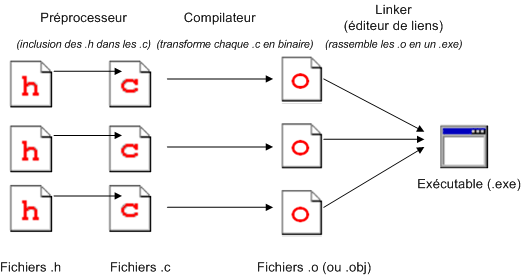
\includegraphics[width=13.5cm]{compilation.png}
	\caption{La compilation}
\end{figure}
\subsection{\'Etape 1 : Le préprocesseur}
Le pré processeur sont les instructions situés en dehors d'un programme, ceux-ci sont préfixé par un dièse (\#).
\begin{description}
	\item[Entrée] fichier.c
	\item[Sortie] fichier obtenu une fois les modifications effectués.
\end{description}~
\begin{lstlisting}[language=C, caption=Exemple d'instructions pré-processeurs]
#include // remplace par le continu du fichier inclus
#define Arg1 Arg2 // remplace syntaxique de Arg1 par Arg2
\end{lstlisting}
\subsection{Etape 2 : La compilation}
\begin{description}
	\item[Entrée] fichier.c, fichier.h
	\item[Sortie] fichier.o 
\end{description}
\begin{lstlisting}[language=bash]
gcc -c fic1.c fic2.c fic3.c # Créé les fichiers .c
gcc *.o nomExe #Créer l'executable.
\end{lstlisting}
\remarque{La compilation sera étudiée en détails lors des cours de L3 et M1}
\subsection{\'Etape 3 : L'édition de liens}
Rassemble tous les fichiers binaires .o en un seul executable.
\chapter{Exercice}
\'Ecrire un programme qui lit une série de 10 valeurs et affiche la position du minimum et du maximum de la série.
\section{\'Etape 1: Analyser le problème}
\begin{enumerate}
	\item Lire les valeurs
	\item calculer les min et max
	\item afficher le résultat
\end{enumerate}
\section{\'Etape 2: Spécifier les sous-problèmes}
Identifier les entrée, les sorties et leurs propriétés.
\subsection{\texttt{LireLesValeurs}}
\begin{description}
	\item[Entrée] Nombre, les valeurs à lire
	\item[Sortie] Tableau contenant les valeurs lues
\end{description}
\subsection{\texttt{CalculerMinEtMax}}
\begin{description}
	\item[Entrée] Le tableau des valeurs et le nombre de valeur 
	\item[Sortie] Position, min et max. 
\end{description}
\newpage
\section{\'Etape 3: Le code}
\lstinputlisting[language=C, caption=Code du programme]{exo1.c}
	\appendix
	\chapter{Glossaire}
	\paragraph{Compilation} Un compilateur est un programme informatique qui transforme un code source écrit dans un langage de programmation (le langage source) en un autre langage informatique (le langage cible).
	\paragraph{Interprétation}
	Analyse, traduit et exécute un programme écrit dans un langage informatique. De tels langages sont dits langages interprétés.

	L'interpréteur est capable de lire le code source d'un langage sous forme de script, habituellement un fichier texte, et d'en exécuter les instructions après une analyse syntaxique du contenu. Généralement ces langages textuels sont appelés des langages de programmation. Cette interprétation conduit à une exécution d'action ou à un stockage de contenu ordonné par la syntaxe textuelle.
	\paragraph{Édition de liens} Lors d’un développement informatique, l'édition des liens est un processus qui permet de créer des fichiers exécutables ou des bibliothèques dynamiques ou statiques, à partir de fichiers objets.
	\lstlistoflistings{}
\end{document}






